\documentclass[10pt,letterpaper]{article}

\usepackage[margin=.5in]{geometry}
%\usepackage{xfrac}
\usepackage{polynom}
\usepackage{tikz}
\usepackage{amsmath}
\usepackage{pgfplots}

\usetikzlibrary{calc}
\newcommand{\tikzmark}[1]{\tikz[overlay,remember picture] \node (#1) {};}

\begin{document}
%\everymath{\scriptscriptstyle}
\parindent=0pt
\abovedisplayshortskip=0pt
\belowdisplayshortskip=0pt
\abovedisplayskip=0pt
\belowdisplayskip=0pt
%% \fbox{\begin{minipage}{92pt}
%% \centering Quadratic Formula
%% $$
%% x = \frac{-x \pm \sqrt{b^2 - 4ac}}{2a}
%% $$
%% \end{minipage}}
\fbox{\begin{minipage}{60pt}
    \centering Square Roots
    \[
    \sqrt{x^6} = |x^3|
    \] \[
    \sqrt{x^8} = x^4
    \] \[
    \sqrt{x^7} = x^3\sqrt{x}
    \]
\end{minipage}}
\fbox{\begin{minipage}{130pt}
    \centering Absolute Value Inequalities
    \[
    \begin{array}{l l}
      |x| < c & \quad -c < x < c\\
      |x| > c & \quad x < -c \textrm{~or~} c < x
    \end{array}
    \]
\end{minipage}}
%\hspace{5pt}
\fbox{\begin{minipage}{157pt}
    \centering Distance Formula
    \[
    A(x_1,y_2) \textrm{~and~} B(x_2, y_2)
    \]
    %\vspace*{-20pt} 
    \[
    d(A, B) = \sqrt{(x_2 - x_1)^2 + (y_2 - y_1)^2}
    \]
\end{minipage}}
\fbox{\begin{minipage}{102pt}
    \centering Midpoint Formula
    \[
    A(x_1,y_2) \textrm{~and~} B(x_2, y_2)
    \]
    %\vspace*{-20pt} 
    \[
    \left( \frac{x_1 + x_2 }{2} , \frac{y_1 + y_2 }{2} \right)
    \]
\end{minipage}}

\fbox{\begin{minipage}{93pt}
    \centering Equation of a Circle
    \[
    (x - h)^2 + (y - k)^2 = r^2
    \]
\end{minipage}}
\fbox{\begin{minipage}{77pt}
    \centering Point-Slope Form
    \[
    y - y_1 = m(x - x_1)
    \]
\end{minipage}}
%% \fbox{\begin{minipage}{95pt}
%% \centering Slope-Intercept Form
%% $$
%% y = mx + bb
%% $$
%% \end{minipage}}
\fbox{\begin{minipage}{68pt}
    \centering Standard Form
    \[
    Ax + By + C = 0
    \]
\end{minipage}}
\fbox{ \begin{minipage}{140pt}
    \centering All Students Take Calculus

    I--All pos. II--sin III--tan IV--cos
\end{minipage}}
\fbox{ \begin{minipage}{96pt}
    \centering Law of Cosines
    \[
    a^2=b^2+c^2-2bc\cdot\cos A
    \]
\end{minipage}}

\fbox{\begin{minipage}{65pt}
    \centering Joint Variation

    \scriptsize \linespread{.5} If $z$ is varies jointly as $x$ and $y$,\normalsize \linespread{1}
    \vspace*{-5pt}
    \[
    z=kxy
    \]
\end{minipage}}
%% \abovedisplayshortskip=0pt
%% \belowdisplayshortskip=0pt
%% \abovedisplayskip=0pt
%% \belowdisplayskip=0pt
\fbox{\begin{minipage}{61pt}
    \centering Perpendicular Lines
    \[
    m_2 = - \frac{1}{m_1}
    \]
\end{minipage}}
\fbox{\begin{minipage}{158pt}
    \centering Average Rate of Change
    \[
    \textrm{ARoC} = \frac{\textrm{y change}}{\textrm{x change}} = \frac{f(x_2) - f(x_1)}{x_2-x_1}
    \]
\end{minipage}}
\fbox{\begin{minipage}{117pt}
    \centering Difference of Cubes
    \[
    a^3+b^3=(a+b)(a^2-ab+b^2)
    \] \[
    a^3-b^3=(a-b)(a^2+ab+b^2)
    \]
\end{minipage}}
\fbox{\begin{minipage}{90pt}
    \centering Standard Form of a Quadratic Function
    \[
    f(x) = a(x-h)^2 + k
    \]
\end{minipage}}

\fbox{\begin{minipage}{210pt}
    \centering Vertical Shifts of Graphs

    \raggedright Suppose $c > 0$.

    Graph $y = f(x) + c$ by shifting $y = f(x)$ up $c$.

    Graph $y = f(x) - c$ by shifting $y = f(x)$ down $c$.
\end{minipage}}
\fbox{\begin{minipage}{210pt}
    \centering Horizonal Shifts of Graphs

    \raggedright Suppose $c > 0$.

    Graph $y = f(x - c)$ by shifting $y = f(x)$ right $c$.

    Graph $y = f(x + c)$ by shifting $y = f(x)$ left $c$.
\end{minipage}}
\fbox{\begin{minipage}{44pt}
    \centering Definition of Log
    \[
    \textrm {if~} a^x = y,
    \] \[
    \log_ay=x
    \]
\end{minipage}}
\fbox{ \begin{minipage}{31pt}
    \centering Arc Length
    \[
    s=r\theta
    \]
\end{minipage}}

\fbox{\begin{minipage}{235pt}
    \centering Reflecting Graphs

    \raggedright
    Graph $y = -f(x)$ by reflecting $y = f(x)$ in the $x$-axis.

    Graph $y = f(-x)$ by reflecting $y = f(x)$ in the $y$-axis.
\end{minipage}}
\fbox{ \begin{minipage}{211pt}
    \centering Vertical Stretching of Graphs

    \raggedright To graph $y = cf(x)$, graph $y = f(x)$, then
    \[
    \begin{array}{rl}
      \textrm{if~} c > 1 & \textrm{strech vertically a by factor of $c$}\\
      \textrm{if~} 0 < c < 1 & \textrm{shrink vertically a by factor of $c$}
    \end{array}
    \]
\end{minipage}}
\fbox{\begin{minipage}{65pt}
    \centering Inverse Variation

    \scriptsize \linespread{.5} If $y$ is inversly proportional to $x$,\normalsize \linespread{1}
    \vspace*{-5pt}
    $y = \frac{k}{x}$
    \vspace*{5pt}
\end{minipage}}

\fbox{ \begin{minipage}{227pt}
    \centering Horizontal Stretching of Graphs

    \raggedright To graph $y = f(cx)$, graph $y = f(x)$, then
    \[
    \begin{array}{rl}
      \textrm{if~} c > 1 & \textrm{shrink horizontally by a factor of $\frac{1}{c}$}\\
      \textrm{if~} 0 < c < 1 & \textrm{stretch horizontally by a factor of $\frac{1}{c}$}
    \end{array}
    \]
\end{minipage}}
\fbox{ \begin{minipage}{150pt}
    \centering Even and Odd Functions
    \[
    \begin{array}{rl}
      \textrm{if~} f(-x)=f(x) & \textrm{$f(x)$ is even}\\
      \textrm{if~} f(-x)=-f(x) & \textrm{$f(x)$ is odd}
    \end{array}
    \]
\end{minipage}}
\fbox{ \begin{minipage}{124pt}
    \centering Heron's Formula
    \[
    A=\sqrt{s(s-a)(s-b)(s-c)}
    \]
\end{minipage}}

\fbox{ \begin{minipage}{151pt}
    \centering Min or Max of a Quadratic Function
    \[
    \begin{array}{rl}
      f(x) = x(x-h)^2 + k & f(h)=k\\
      f(x) = ax^2+bx+c & \textrm{$f(-\frac{b}{2a})$}
    \end{array}
    \]
\end{minipage}}
\fbox{ \begin{minipage}{67pt}
    \centering Change of Base
    \[
    \log_bm=\frac{\log m}{\log b}
    \]
\end{minipage}}
\fbox{ \begin{minipage}{69pt}
    \centering Completing the Square

    \scriptsize \linespread{.5} With a quadratic in form $ax^2 + bx = c$ \normalsize \linespread{1}
    %\vspace*{-5pt}

    $(\frac12 \cdot b)^2 = c$
    %\vspace*{5pt}
\end{minipage}}
\fbox{ \begin{minipage}{88pt}
    \centering Hidden quadratic 1
    \[
    x^{-3/2}+2x^{-1/2}+x^{1/2}
    \]\[
    x^{-3/2}(1+2x+x^2)
    \]\[
    x^{-3/2}(1+x)^2
    \]
\end{minipage}}
\fbox{ \begin{minipage}{60pt}
    \centering Hidden quadratic 2
    \[
    e^{2x}+2e^x+1
    \]\[
    (e^x+1)^2
    \]
\end{minipage}}

\fbox{ \begin{minipage}{78pt}
    \centering Permutations
    \[
    p(x,y)=\frac{x!}{(x-y)!}
    \]
\end{minipage}}
\fbox{ \begin{minipage}{123pt}
    \centering Choose Formula
    \[
    C(x,y)= {x\choose y}=\frac{x!}{y!(x-y)!}
    \]
\end{minipage}}
\fbox{ \begin{minipage}{100pt}
    \centering Law of Sines
    \[
    \frac{\sin A}{a} = \frac{\sin B}{b} = \frac{\sin C}{c}
    \]
\end{minipage}}
\fbox{ \begin{minipage}{84pt}
    \centering Degrees to Radians
    \[
    \frac{A\cdot\pi}{180}=\theta
    \]
\end{minipage}}
\fbox{ \begin{minipage}{90pt}
    \centering Remainder Theorem

    \raggedright If $P(x) \div (x-c)$, the remainder $= P(c)$.
\end{minipage}}

\fbox{ \begin{minipage}{159pt}
    \centering SOH-CAH-TOA
    \[
    \sin=\frac{\textrm{opp}}{\textrm{hyp}} \quad
    \cos=\frac{\textrm{adj}}{\textrm{hyp}} \quad
    \tan=\frac{\textrm{opp}}{\textrm{adj}}
    \]
\end{minipage}}
\fbox{ \begin{minipage}{52pt}
    \centering Sector Area
    \[
    A=\frac12r^2\theta
    \]
\end{minipage}}
\fbox{\begin{minipage}{65pt}
    \centering Direct Variation

    \scriptsize \linespread{.5} If $y$ is directly proportional to $x$,\normalsize \linespread{1}
    \vspace*{-5pt}
    \[
    y = kx
    \]
\end{minipage}}
\fbox{ \begin{minipage}{90pt}
    \centering Population Growth

    \raggedright \footnotesize n is population size, r is relative growth rate, t is time

    \normalsize\vspace*{-20pt}
    \[
    n=n_0e^{rt}
    \]
\end{minipage}}
\fbox{\begin{minipage}{70pt}
    \centering Area of $\Delta$
    \[
    A = ab\cdot \frac12 \sin C
    \]
\end{minipage}}

\fbox{ \begin{minipage}{140pt}
    \centering Property of logs
    \[
    (\log_ab)(\log_cd)=(\log_ad)(\log_cb)
    \]
\end{minipage}}
\newpage
\fbox{\begin{minipage}{266pt}
    \centering Algebra of Functions

    \raggedright Let $f$ and $g$ be functions with domains $A$ and $B$.
    \[
    \begin{array}{cl}
      (f+g)(x)=f(x)+g(x) & \textrm{Domain~} A \cap B  \\
      (f-g)(x)=f(x)-g(x) & \textrm{Domain~} A \cap B \\
      (fg)(x)=f(x)g(x) & \textrm{Domain~} A \cap B \\
      \left(\frac{f}{g}\right)(x)=\frac{f(x)}{g(x)} & \textrm{Domain~} \{x \in A \cap B \mid g(x) \neq 0\} \\
      (f \circ g)(x)=f(g(x)) & \textrm{Domain~} \{x \in B \mid g(x) \in A\}
    \end{array}
    \]
\end{minipage}}
\fbox{\begin{minipage}{133pt}
    \centering Polynomial Synthetic Division
    \[
    (x^3+x^2-1) \div (x+2)
    \]
    \polyset{showbase=top}
    \hspace{-7pt}\polyhornerscheme[x=-2,stage=8]{x^3+x^2-1}
\end{minipage}}
\fbox{\begin{minipage}{118pt}
    \centering Polynomial Long Division
    \polylongdiv[stage=8]{x^3+x^2-1}{x+2}
\end{minipage}}

\fbox{\begin{minipage}{140pt}
    \centering Rational Roots Theorem
    \[
    2x^3+2x^2-3x-6
    \] 
    \hspace{15pt}$\pm1, \pm2$ \hfill $\pm1, \pm2, \pm3, \pm6$

    Possible rational roots:

    $\pm1, \pm\frac{1}{2}, \pm2, \pm3, \pm\frac{3}{2}, \pm6$
\end{minipage}}
\fbox{\begin{minipage}{140pt}
    \centering Decartes' Rule of Signs

    \raggedright Count num. of sign changes
    \[
    P(x)=3x^6+4x^5+\tikzmark{a}3x^3-\tikzmark{b}x-3
    \begin{tikzpicture}[overlay,remember picture,out=315,in=225,distance=0.4cm]
      \draw[-latex] (a) to (b);
    \end{tikzpicture}
    \]
    1 positive real root
    \[
    P(-x)=\tikzmark{a}3x^6-\tikzmark{b}4x^5-\tikzmark{c}3x^3+\tikzmark{d}x-\tikzmark{e}3
    \begin{tikzpicture}[overlay,remember picture,out=315,in=225,distance=0.4cm]
      \draw[-latex] (a) to (b);
      \draw[-latex] (c) to (d);
      \draw[-latex,out=290,in=250] (d) to (e);
    \end{tikzpicture}
    \vspace*{5pt}
    \]
    1 or 3 negative real roots
\end{minipage}}
\fbox{\begin{minipage}{140pt}
    \centering Logarithm Formulas
    \begin{align*}
      \log(m\cdot n) &= \log m + \log n \\
      \log\left(\frac{m}{n}\right) &= \log m - \log n \\
      \log(m^n) &= n \cdot \log m \\
      \log_bb^x &= x =b^{\log_bx} 
    \end{align*}
\end{minipage}}
\fbox{\begin{minipage}{67pt}
    \centering Other trig stuff
    \begin{align*}
      \cot &= \frac1{\tan} \\
      \csc &= \frac1{\sin} \\
      \sec &= \frac1{\cos}
    \end{align*}
\end{minipage}}

\fbox{\begin{minipage}{216pt}
    \centering Horizontal Asymptotes
    \begin{align*}
      y&=\frac{2x^2-4x+5}{x^2-2x+1} &&\, \textrm{Original Equation}\\
      &=\frac{2x^2}{x^2} &&\, x \to \infty, \textrm{other terms $\to$ tiny}\\
      &=2 &&\, \textrm{Cancel, horizontal asymptote}
    \end{align*}
\end{minipage}}
\fbox{\begin{minipage}{212pt}
    \centering Slant Asymptotes
    \begin{align*}
      y&=\frac{x^2-4x-5}{x-3} &&\, \textrm{Original Equation}\\
      &=x-1-\frac{8}{x-3} &&\, \textrm{Divide}\\
      &=x-1 &&\, x\to\infty, \textrm{other terms $\to$ tiny}
    \end{align*}
\end{minipage}}

\fbox{\begin{minipage}{181pt}
    \centering Vertical Asymptotes
    \begin{align*}
      y&=\frac{2x^2-4x+5}{x^2-2x+1} &&\, \textrm{Original Equation}\\
      &=\frac{2x^2-4+5}{(2x-1)(x+2)} &&\, \textrm{Factor demoniator}\\
      x&=\frac12 \textrm{~or~} x=-2 &&\, \textrm{Impossible}
    \end{align*}
\end{minipage}}
\fbox{\begin{minipage}{152pt}
    \centering End Behavior

    \begin{minipage}{40pt}
      \[
      y=x^n
      \]
      $n$ is even\vspace{5pt}
      \[
      y=x^n
      \]
      $n$ is odd
    \end{minipage}
    \begin{minipage}{30pt}
      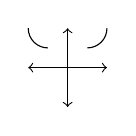
\begin{tikzpicture}
        \draw[<->] (-.5,0) -- (.5,0);
        \draw[<->] (0,-.5) -- (0,.5);
        \draw[in=270,out=0] (.25,.25) to (.5,.5);
        \draw[in=270,out=180] (-.25,.25) to (-.5,.5);
      \end{tikzpicture}
      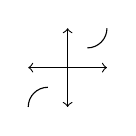
\begin{tikzpicture}
        \draw[<->] (-.5,0) -- (.5,0);
        \draw[<->] (0,-.5) -- (0,.5);
        \draw[in=270,out=0] (.25,.25) to (.5,.5);
        \draw[in=90,out=180] (-.25,-.25) to (-.5,-.5);
      \end{tikzpicture}
    \end{minipage}~
    \begin{minipage}{40pt}
      \[
      y=-x^n
      \]
      $n$ is even\vspace{5pt}
      \[
      y=-x^n
      \]
      $n$ is odd
    \end{minipage}
    \begin{minipage}{30pt}
      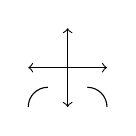
\begin{tikzpicture}
        \draw[<->] (-.5,0) -- (.5,0);
        \draw[<->] (0,-.5) -- (0,.5);
        \draw[in=90,out=0] (.25,-.25) to (.5,-.5);
        \draw[in=90,out=180] (-.25,-.25) to (-.5,-.5);
      \end{tikzpicture}
      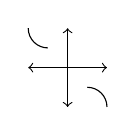
\begin{tikzpicture}
        \draw[<->] (-.5,0) -- (.5,0);
        \draw[<->] (0,-.5) -- (0,.5);
        \draw[in=90,out=0] (.25,-.25) to (.5,-.5);
        \draw[in=270,out=180] (-.25,.25) to (-.5,.5);
      \end{tikzpicture}
    \end{minipage}
\end{minipage}}
\fbox{ \begin{minipage}{77pt}
    \centering Trig Identities
    \begin{align*}
      \sin^2+\cos^2&=1\\
      \tan^2 + 1 &= \sec^2\\
      1+\cot^2&=\csc^2
    \end{align*}
\end{minipage}}

\fbox{\begin{minipage}{183pt}
    \centering $y=\sin x$ in red; $y=\cos x$ in blue
    
    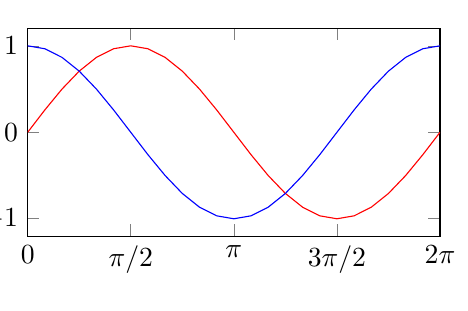
\begin{tikzpicture}[trim axis left,trim axis right]
      \begin{axis}[domain=0:2*pi,xmin=0,xmax=6.28318,ymin=-1.2,ymax=1.2,width=194pt,height=120pt,xtick={0,1.570795,3.14159,4.712385,6.28318},xticklabels={0,$\pi/2$,$\pi$,$3\pi/2$,$2\pi$}]
        \addplot[red] plot (\x, {sin(\x r)});
        \addplot[blue] plot (\x, {cos(\x r)});
      \end{axis}

    \end{tikzpicture}
\end{minipage}}
\fbox{\begin{minipage}{183pt}
    \centering $y=\csc x$ in red; $y=\sec x$ in blue, asymtotes dotted
    
    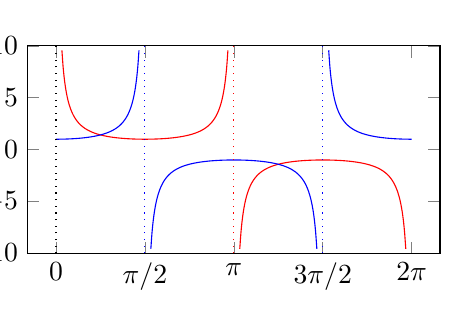
\begin{tikzpicture}[trim axis left,trim axis right]
      \begin{axis}[domain=0:2*pi,xmin=-0.5,xmax=6.78318,ymin=-10,ymax=10,restrict y to domain=-10:10,width=194pt,height=120pt,xtick={0,1.570795,3.14159,4.712385,6.28318},xticklabels={0,$\pi/2$,$\pi$,$3\pi/2$,$2\pi$}]
        \addplot[smooth,red,samples=301] plot (\x, {cosec(\x r)});
        \addplot[smooth,blue,samples=301] plot (\x, {sec(\x r)});
        \draw[dotted] (axis cs:0,-10) -- (axis cs:0,10);
        \draw[blue,dotted] (axis cs:1.570795,-10) -- (axis cs:1.570795,10);
        \draw[red,dotted] (axis cs:3.14159,-10) -- (axis cs:3.14159,10);
        \draw[blue,dotted] (axis cs:4.712385,-10) -- (axis cs:4.712385,10);
      \end{axis}

    \end{tikzpicture}
\end{minipage}}
\fbox{ \begin{minipage}{140pt}
    \centering sin/cos/csc/sec Graph Properties

    \raggedright If in form:
    \[
    y=a\sin k(x-b)
    \]
    amplitude  $|a|$, period  $2\pi/k$, phase shift $b$
\end{minipage}}
\end{document}
